\RequirePackage[dvipsnames]{xcolor}
\documentclass[10pt]{NSP1}
\usepackage{url,floatflt}
\usepackage{helvet,times}
\usepackage{psfig,graphics,graphicx}
\usepackage{mathptmx,amsmath,amssymb,bm}
\usepackage{float}
\usepackage[bf,hypcap]{caption}
\usepackage{subcaption}
\usepackage{soul}
\usepackage{listings}
\usepackage{booktabs}
\usepackage{siunitx}
\usepackage{multirow}
\usepackage{tabularx}
\setlength{\tabcolsep}{3pt}


\tolerance=1
\emergencystretch=\maxdimen
\hyphenpenalty=10000
\hbadness=10000

\topmargin=0.00cm

\def\sm{\smallskip}
\def\no{\noindent}

\def\firstpage{1}
\setcounter{page}{\firstpage}
\def\thevol{20}
\def\thenumber{5}
\def\theyear{2026}


\begin{document}

\titlefigurecaption{{\large \bf \rm Applied Mathematics \& Information Sciences }\\ {\it\small An International Journal}}

\title{A Random Survival Forest Model for Time-to-Virologic Failure and Drug Resistance: Randomized Factorial Design using Data from Botswana}

\author{Claris Shoko{$^1$}, Kesaobaka Molebatsi{$^2$}, Katleho Makatjane{$^3$}, Ontlametse Thato Choga{$^2$}, Sikhulile Moyo{$^{4,5,6,7}$}}
\institute{$^1$Department of Statistics, Faculty of Social Sciences, University of Botswana, Botswana. \\
$^2$Botswana Harvard Health Partnership, Botswana.\\
$^3$Department of Statistics and Population Studies, University of the Western Cape, South Africa.\\
$^4$School of Allied Health Sciences, Faculty of Medicine and Health Sciences, University of Botswana, Botswana.\\
$^5$Department of Immunology and Infectious Diseases, Harvard T.H. Chan School of Public Health, Boston, MA, United States,\\
$^6$School of Health Systems and Public Health, University of Pretoria, Pretoria, South Africa,\\
$^7$Division of Medical Virology, Faculty of Medicine and Health Sciences, Stellenbosch University, Tygerberg, South Africa}

\titlerunning{Random Survival Forest for Time to Virologic Failure}
\authorrunning{C. Shoko et al.}

%corresponding author email
\mail{shokoc@ub.ac.bw}

\received{...}
\revised{...}
\accepted{...}
\published{...}

\abstracttext{We analyse the clinical and drug-related factors that predict time to treatment failure and development of drug resistance among people living with HIV (PLWH). We demonstrate this on an open-label, randomized, $3 \times 2 \times 2$ factorial design study that was conducted in Botswana from 2002 to 2007, involving 650 antiretroviral therapy (ART)-naïve individuals. To identify predictors associated with virologic failure and drug resistance, variables were initially pre-screened using the log-rank test. A Random Survival Forest (RSF) model was built with the log-rank splitting rule and 80 trees. The model's performance was assessed using Brier scores, out-of-bag error, concordance index (C-index) and continuous ranked probability scores (CRPS). To further examine variable importance and interaction effects, paired variable significance measures and maximum subtree depth were also analyzed. The RSF model showed excellent prediction accuracy, with ensemble survival probability over 90\% and low Brier scores across all risk percentiles. The key predictors of virologic failure were the non-nucleoside transcriptase inhibitors (NRTI) class, treatment arm, baseline CD4 count of 250 cells/mm³ or less, World Health Organisation (WHO) HIV/AIDS clinical stage 4 (severe symptoms), severe anemia, and wasting syndrome. While Stavudine/Lamivudine (D4T/3TC)-based regimens were associated with a low risk of virologic failure and drug resistance, Zidovudine/Didanosine (ZDV/ddI)-containing regimens were associated with a higher risk of virologic failure and drug resistance. We found a significant interaction between drug regimens and clinical stage. The probabilities of survival from virologic failure with resistance increased with time on treatment. Random Survival Forest provides a robust and flexible tool for survival analysis in HIV research, showing significant handling complex interactions. The findings support risk-based patient monitoring and regimen optimization to enhance virologic suppression for people living with HIV (PLWH)..}

\keywords{Antiretroviral Regimen Evaluation, Censored Time-to-Event Data, Clinical Decision Support Systems, Machine Learning in Public Health, Virologic Failure.}

\maketitle

\section{Introduction}

The HIV/AIDS pandemic continues to be a major public health challenge globally. Despite treatment advancements and prevention strategies, millions of people living with HIV (PLWH) continue to face challenges. A report by UNAIDS \cite{UNAIDS2024}shows that in 2023, 1.3 million new infections were recorded globally, increasing the number of PLWH to 40.8 million. However, among PLWH, about 9.2 million were not accessing antiretroviral therapy (ART), which is crucial for viral load (VL) suppression and preventing onward transmission. The African region has been disproportionately affected by the HIV pandemic. Sub-Saharan Africa bears the global HIV/AIDS pandemic, with over 70\% of PLWH globally. This burden translates to high rates of new infections, AIDS-related deaths and a rise in orphaned children. In 2022, Sub-Saharan Africa recorded 760,000 new infections and 380,000 deaths due to AIDS-related illnesses \cite{WHO2023}.

Despite the use of potent ART, there is still a subset of PLWH experiencing virologic failure (VF) rather than complete viral suppression \cite{Bareng2024}. VF occurs when ART fails to suppress and sustain a person's VL to less than the lower limit of the detection assay, depending on the HIV treatment guidelines utilised in a specific setting. Multiple factors may play a role in the development or increased risk of progression to VF. Different cohort studies have shown that suboptimal adherence frequently plays a major role in the development of VF \cite{Daltro2023}; \cite{Ekstrand2011}. Other factors associated with VF included problems with pharmacokinetics (inadequate absorption, underdosing, and drug interactions) \cite{Bulage2017}; \cite{Chun2010}; \cite{Tobin2005}. VF has also been attributed to accumulation of  HIV drug resistance mutations \cite{Manakhov2025}; \cite{Li2021}. The ongoing replication of ART produces new virions, which, in some cases, result in a mutated virus. This will keep on driving the HIV infection and fueling the HIV disease progression, including the development of opportunistic infections such as Tuberculosis (TB) and anemia. 

Several studies have investigated time-to-event outcomes and their determinants among PLWH, predominantly using the Cox Proportional Hazards model. For instance, Naghibifar et al. (2024) assessed the survival of PLWH, co-infections, and other related factors using the Cox proportional hazard model. Similarly, Isingo et al (2007) examined post-HIV survival in a rural Tanzanian cohort during the ART era. These studies employed Kaplan-Meier survival functions and estimated median survival time using Weibull models, reporting an overall survival rate of 67%.

 In Southern Iran, \cite{Afrashteh2023} used a Cox regression model to investigate the survival for PLWH on ART, where a 2-year survival rate was 87\%. Additionally, \cite{Pu2024} applied both the univariate and multivariate Cox proportional hazard model to examine the factors associated with survival after ART initiation, aiming to inform treatment strategies and prognosis improvement strategies for PLWH. Other similar studies include the study by \cite{Nigussie2020}, \cite{Nura2024}, and a recent study by \cite{Shaik2025}, all of which utilized Cox-based survival methods to determine survival rate and identify the predictive factors. 
 
Nevertheless, machine learning approaches, particularly Random Survival Forest (RSF), have overtaken the classical methods, including the Cox Proportional Hazards. The most significant limitation of the Cox PH model is its core assumption that the hazard ratio between any two individuals is constant over time. RSF does not rely on this assumption, allowing it to model situations where the effect of a covariate changes over time. If the proportional hazards assumption is violated, the Cox model can produce biased estimates and unreliable predictions. The assumption of a constant hazard ratio between two groups can be restrictive and unrealistic in many real-world scenarios. RSFs can assess the importance of different variables in predicting survival \cite{Breiman2003}. RSF's tree-based ensemble approach is more flexible than the semi-parametric structure of the Cox model, leading to higher predictive accuracy in many scenarios that include 1) automatic interaction detection, 2) robust to non-linearity, 3) superior for complex data. RSF includes a built-in validation mechanism and methods for evaluating variable importance, that is the Out-of-Bag (OOB) error used to estimate prediction error and the variable importance (VIMP) that automatically ranks the importance of each variable in its predictions, thereby providing insight into the most influential factors. However, relatively few studies used machine learning approaches to evaluate time-to-event outcomes. \cite{Nasejje2017} compared the Cox proportional hazard model with the RSF in analyzing mortality among under-five-year-old children in Uganda. Their findings were supportive of RSF over the Cox proportional hazard model. 

RSF is an ensemble method that builds/combines multiple decision trees to make predictions \cite{Breiman2003}. Each tree is trained on a slightly different subset of data (bootstrap samples) and uses random selection of features at each split. Survival trees predict a survival function, for example, the probability of surviving past a certain time. The splitting criteria used to determine how to divide data at each node are the log-rank or log-rank score test. A comparison of these two splitting criteria can be done to find out which of the two outperforms the other. The Out-Of-Bag (OOB) error is a key feature of random forest \cite{Ishwaran2008}. In bootstrap sampling, some features are left out for each tree, and these can be used to estimate the model’s prediction error without the need for a separate test. Thus, the OOB error estimate is a measure of the model’s predictive performance on observed data. Prediction of the new data points is assessed by aggregating predictions from all trees, involving averaging survival curves or using other methods to combine individual tree predictions. The Brier score (BS) is also one of the most widely used metrics to quantify the error in an estimated survival distribution $\hat{S} (t|x_i)$ \cite{Berkowitz2023}, used together with the Concordance-index \cite{Ishwaran2008}. This makes the RSF less prone to overfitting. 

In contrast to recent research by \cite{Naghibifar2024} and \cite{Afrashteh2023}, which examined mortality outcomes through Cox models, the present study specifically addresses VF and resistance, thereby offering a more detailed perspective on early ART outcomes. This study uses a RSF benchmarked to the Cox proportional hazards model to predict the probability of survival from VF and drug resistance among PLWH on treatment. The novelty of this study is the ability to analyse time to VF and drug resistance, while in most studies, the event of interest was mortality. This study goes further to identify interactions between explanatory variables



\section{Materials and Methods}
\subsection{Study Population}


We used data from the Tshepo study, which is an open-label, randomized, $3\times 2 \times 2$ factorial design study conducted at Botswana Harvard Health Partnership in Gaborone, Botswana, from 2002 to 2007. The main study aim was to evaluate the efficacy, tolerability, and the development of drug resistance of six different first-line combination antiretroviral therapy (cART) regimens among adults living with HIV. The evaluated regimens were: ZDV/3TC/NVP (Arm 1); ZDV/3TC/EFV (Arm 2); ZDV/ddI/NVP (Arm 3); ZDV/ddI/EFV (Arm 4); d4T/3TC/NVP (Arm 5), and d4T/3TC/EFV (Arm 6) (where ZDV= Zidovudine, 3TC= Lamivudine, NVP= Nevirapine, EFV= Efavirenz, DDI=Dianosine, d4T= Stavudine). The study further compared two different adherence strategies: standard-of-care (SOC) versus standard-of-care plus community-based supervision (Com-DOT) to determine the better method for promoting adherence among treatment-naïve adults initiating cART. Adults ($\geq$18 years of age), living with HIV, cART-naïve, Botswana citizens who attended one of the five ART screening clinics in Gaborone were approached for possible enrollment. All potentially eligible adults had to qualify for cART, based on existing Botswana National ARV Treatment guidelines (Ministry of Health, Botswana; 2002) of having an AIDS-defining illness and/or CD4\textsuperscript{+} T cell count $\geq 200$ cells/mm$^3$ or meet this study's upper CD4 stratum eligibility criteria which was a CD4\textsuperscript{+} T cell count between 201 and 350 cells/mm$^3$ with plasma HIV-1 RNA level $\geq 55$,000 copies/mL. Potentially eligible adults also had to reside within the study catchment area for the duration of the study. Other inclusion criteria were as follows: hemoglobin value greater than 8.0 grams/dL; absolute neutrophil count greater than or equal to $1.0 \times $ 103/mm$^3$; aminotransferase levels less than five times the upper limit of the normal; serum alkaline phosphatase level of less than three times the upper limits of the normal; and for women of child-bearing potential, a willingness to maintain active contraception throughout the duration of the study and a negative urine pregnancy test within 14 days of study enrollment. Exclusion criteria were: poor Karnofsky performance score (40 or below); an AIDS-related malignancy other than mucocutaneous Kaposi's sarcoma; grade 2 or higher peripheral neuropathy; major psychiatric illness; and, for women, actively breastfeeding and/or less than six months post-partum \cite{Bussmann2009}.

\subsection{Ethical Approval}
Ethical review board approval was obtained from the Ministry of Health, Botswana (Health Research Development Committee) and the Harvard School of Public Health (Human Subjects Committee). The study participants consented for their clinical data and samples to be used in future studies. The "Tshepo study" in Botswana has an identifier number of NCT03806788.

\subsection{Data Description}
A sample of 650 PLWH were randomly assigned to 6 treatment arms, a combination of the nucleotide reverse transcriptase inhibitors (NRTI) and non-NRTI (NNRTI). From the 650 individuals, treatment was randomly assigned as follows: 109 individuals were given a triple therapy consisting of NVP/ZDV/3TC-ta1, 108 were administered with NVP/ZDV/ddI-ta3, 108 with NVP/D4T/3TC-ta5, 109 with EFV/ZDV/3TC-ta2, 108 with EFV/ZDV/ddI-ta4, and another 108 with EFV/D4T/3TC-ta6. This shows an even distribution of PLWH across all treatment combinations. The distribution of the 6 treatment arms is presented in Table \ref{tab:treatmentarms}

\begin{table}[H]
    \centering
    \caption{The 6 Treatment Arms from a combination of 2 NNRTI class and 3 NRTI class of ART regimens}
    \label{tab:treatmentarms}
    \begin{tabular}{|c|c|c|c|c|c|c|c|}
        \toprule
        \multicolumn{2}{c|}{\textbf{Treatment Arm (ta)}} & \textbf{1} & \textbf{2} & \textbf{3} & \textbf{4} & \textbf{5} & \textbf{6} \\
        \cmidrule(lr){1-2}\cmidrule(lr){3-8}
        \textbf{NNRTI} & \textbf{NRTI} & & & & & & \\
        \midrule
        \multirow{3}{*}{NVP=1} & ZDV/3TC=1 & 109 & 0 & 0 & 0 & 0 & 0 \\
        & ZDV/ddI=2 & 0 & 0 & 108 & 0 & 0 & 0 \\
        & D4T/3TC=3 & 0 & 0 & 0 & 0 & 108 & 0 \\
        \midrule
        \multirow{3}{*}{EFV=2} & ZDV/3TC=1 & 0 & 109 & 0 & 0 & 0 & 0 \\
        & ZDV/ddI=2 & 0 & 0 & 0 & 108 & 0 & 0 \\
        & D4T/3TC=3 & 0 & 0 & 0 & 0 & 0 & 108 \\
        \bottomrule
    \end{tabular}
\end{table}

\subsection{Statistical Analysis }
The RSF model \cite{Breiman2003} was used to determine the factors that predicted time to VF and drug resistance. Pre-screening of the factors was done using the log-rank test (Segal, 1988). Variables with p-values below 10\% in log-rank tests were fitted in the RSF model. For categorical variables, the study analysed how each category relates to virologic outcome, thereby giving insights as to the proper management of treatment. For example, for the treatment arm variable, the fitted model informs as to which treatment arm is associated with the best survival outcome. Data analysis is done using R software version 4.4.1 and the package ‘randomForestSRC’ \cite{Ishwaran2025}.

\subsubsection{Random Survival Forest (RSF): Survival Data Structure}

The training dataset consists of triplets containing features, observed times, and censoring indicators:

\begin{equation}
\mathcal{D} = \{(\mathbf{x}_1, T_1, \delta_1), (\mathbf{x}_2, T_2, \delta_2), \dots, (\mathbf{x}_N, T_N, \delta_N)\}
\end{equation}

\begin{itemize}
    \item $\mathbf{x}_i \in \mathbb{R}^d$: The d-dimensional feature vector for individual $i$.
    \item $T_i = \min(Y_i, C_i)$: The observed time, where $Y_i$ is the true event time and $C_i$ is the censoring time.
    \item $\delta_i \in \{0, 1\}$: The censoring indicator, where $\delta_i = 1$ if the event occurred, and $\delta_i = 0$ if the observation was right-censored.
\end{itemize}


For the RSF growing the Ensemble is done via Bootstrapping. An RSF builds an ensemble of B independent survival trees using bootstrap sampling. This involves drawing B bootstrap samples $\mathcal{D}_b$ ($b = 1, \dots, B$) from the original dataset $\mathcal{D}$ with replacement. Each sample leaves out roughly 37\% of the data, known as the Out-of-Bag (OOB) data, used later for validation. At each node of a survival tree, a random subset of $m \approx \sqrt{d}$ candidate features is selected. The node is split into left (L) and right (R) daughter nodes by maximizing the survival difference between them. The standard metric is the Log-Rank Splitting Criterion. For a proposed split, let $t_1 < t_2 < \cdots < t_m$ be the distinct event times in the parent node. The log-rank test statistic $L(X, c)$ for a feature $X$ at a split value $c$ is: 

\begin{equation}
|V|^{-\frac{1}{2}} \sum_{j=1}^{m} \left( d_{j,L} - \frac{Y_{j,L}}{Y_j} d_j \right)
\end{equation}
Where at each event time $t_j$:
\begin{itemize}
    \item $d_j$: Total events across both daughter nodes.
   \item $d_{j,L}$: Events in the left daughter node.
   \item $Y_j$: Total individuals at risk across both daughter nodes.
   \item $Y_{j,L}$: Individuals at risk in the left daughter node.
 \item $V$: The hypergeometric variance of the event count.
\end{itemize}
The split is chosen by finding the feature and value that maximize this statistic. Trees are grown until a termination rule is met (e.g., a minimum number of unique events $d_0$ in a terminal node). For every terminal node $h$ in tree $b$, we calculate the Nelson-Aalen Cumulative Hazard Function (CHF) estimator using only the individuals who fell into that node:
\begin{equation}
\hat{H}_b(t|\mathbf{x}) = \sum_{t_j \leq t} \frac{d_{j,h}}{Y_{j,h}} \quad \text{for } \mathbf{x} \in h
\end{equation}
where $d_{j,h}$ is the number of events at time $t_j$ in terminal node $h$ and $Y_{j,h}$ is the number of individuals at risk at time $t_j$ in terminal node $h$.


The overall ensemble CHF is the simple average of the estimated CHFs from the terminal nodes where $\mathbf{x}_0$ landed across all trees:
\begin{equation}
\bar{H}_e(t|\mathbf{x}_0) = \frac{1}{B} \sum_{b=1}^{B} \hat{H}_b(t|\mathbf{x}_0).
\end{equation}

Using the mathematical relationship between survival and hazard ($S(t) = \exp(-H(t))$), the ensemble survival probability over time is formulated as:
\begin{equation}
\bar{S}_e(t|\mathbf{x}_0) = \exp \left( -\bar{H}_e(t|\mathbf{x}_0) \right)
\end{equation}

The final output metrics for any given test subject $\mathbf{x}_0$ are generated by aggregating individual tree terminal node estimators:
\begin{align}
\bar{H}_e(t|\mathbf{x}_0) &= \frac{1}{B} \sum_{b=1}^{B} \sum_{t_j \leq t} \frac{d_{j,h(b,\mathbf{x}_0)}}{Y_{j,h(b,\mathbf{x}_0)}}, \\
\bar{S}_e(t|\mathbf{x}_0) &= \exp \left( -\bar{H}_e(t|\mathbf{x}_0) \right).
\end{align}

\subsubsection{Error Metrics}
In survival analysis, estimates of survival functions for each individual are obtained, and the estimated median is extracted. Of interest is 1. the distance between the individuals' estimated and the true survival functions, and 2. The closeness of the estimated medians (point predictors) to the observed times. Let $t_i$ and $c_i$ be the realisations of the survival and censored times, respectively, for subject $i, i = 1, \dots, n$. Let $y_i = \min (t_i, c_i)$ be the observed time, and let $\delta_i = I(t_i \leq c_i)$ denote the observed censoring indicator. Let $x_i = (x_{i1}, \dots, x_{ik})$ denote the observed covariates for the $i\text{th}$ individual. Thus the observed data is denoted by $(y_i, \delta_i, x_i)$.

\subsubsection{Integrated Brier score}

The Brier score (BS) is one of the most widely used metrics to quantify the error in an estimated survival distribution $\hat{S}(t \mid x_i)$ (32,33). The BS for the survival of the $i\text{th}$ individual at time $t$ is given by:
\begin{equation}
BS_i(t) = \left[ I(y_i > t) - \hat{S}(t \mid x_i) \right]^2
\label{eq:brier_score}
\end{equation}


\section{Results and Discussions}
In this section of the study, we present results from the data analysis. Data analysis is performed in 3 stages. The first stage is exploratory data analysis where the descriptive statistics for the covariates of interest and a Mantel-Haenszel test for the association of the covariates with the covariates. This stage identifies the covariates to be included the survival analysis models, Cox proportional and the RSF. In stage two we fit a Cox proportional hazards model to analyse survival from VF and drug resistance (VFR). Finally, in stage three we fit the RSF model and then discuss the findings from these two survival models. 
\subsection{Exploratory data analysis}
Before fitting the survival models to our data, a Log-Rank Test/ Mantel-Haenszel Test was performed to find out which variables contribute significantly to the probability of survival from virologic failure and drug resistance at 10\% level. The variables that contributed significantly were used in the RSF model. The results from the Mantel-Haenszel test are presented in Appendix 3. The results show that WHO clinical stage, VlCD4, weeks on treatment, CD4 $\leq$250, severe anemia, age squared, NRTI, baseline wasting syndrome, and treatment arm contribute significantly to the probability of survival. The RSF model was fitted with these covariates included in the model. However, NNRTI class of regimens was also included because the treatment arm is a combination from both NRTI and NNRTI. 


\subsection{The Cox proportional hazards model}
The Cox proportional hazards model is fitted using the variables that passed the Mantel-Haenszel test, as presented in Appendix 3. 

\begin{table}[H]
    \centering
    \caption{Results from the fitted Cox proportional hazards model and the test for the proportional hazards assumption based on Schoenfeld residuals}
    \label{tab:cox_results}
    \begin{tabular}{l r r r r r}
        \toprule
        \multicolumn{6}{l}{\textbf{Fitted Cox Proportional Hazards Model}} \\
        \midrule
        \textbf{Variable} & \textbf{coef} & \textbf{exp(coef)} & \textbf{se(coef)} & \textbf{z} & \textbf{p-value} \\
        \midrule
        wcs2 & -0.050 & 0.951 & 0.527 & -0.095 & 0.924 \\
        wcs3 & 0.412 & 1.510 & 0.442 & 0.932 & 0.352 \\
        wcs4 & 0.350 & 1.419 & 0.650 & 0.538 & 0.590 \\
        vlcd42 & -1.171 & 0.310 & 0.467 & -2.506 & 0.012 \\
        bws1 & 0.945 & 2.574 & 0.510 & 1.853 & 0.064 \\
        wtrt & -0.0173 & 0.983 & 0.007 & -2.561 & 0.011 \\
        sane1 & 0.655 & 1.926 & 0.363 & 1.804 & 0.071 \\
        nnrtita2 & 0.775 & 2.170 & 1.230 & 0.630 & 0.529 \\
        nrtita2 & -0.003 & 0.997 & 1.327 & -0.003 & 0.998 \\
        nrtita3 & -1.746 & 0.174 & 1.074 & -1.626 & 0.104 \\
        ta2 & -1.054 & 0.349 & 1.385 & -0.761 & 0.447 \\
        ta3 & 1.179 & 3.252 & 1.294 & 0.912 & 0.362 \\
        ta4 & NA & NA & 0 & NA & NA \\
        ta5 & NA & NA & 0 & NA & NA \\
        ta6 & NA & NA & 0 & NA & NA \\
        age& -0.005 & 0.995 & 0.021 & -0.262 & 0.793 \\
        cd4$<$250& 0.174 & 1.190 & 0.369 & 0.470 & 0.638 \\
        \midrule
        \multicolumn{6}{l}{\textbf{Test for Proportional Hazards Assumption}} \\
        \midrule
        \textbf{Variable} & \textbf{chisq} & \textbf{df} & \textbf{p-value} & & \\
        \midrule
        wcs & 6.633 & 3 & 0.085 & & \\
        vlcd4 & 1.363 & 1 & 0.243 & & \\
        bws & 0.070 & 1 & 0.791 & & \\
        wtrt & 0.550& 1 & 0.458 & & \\
        sane& 0.051 & 1 & 0.821 & & \\
        nnrtita & 5.239 & 1 & 0.022 & & \\
        nrtita & 3.517 & 2 & 0.172 & & \\
        ta& 8.387 & 5 & 0.015 & & \\
        age & 0.005 & 1 & 0.946 & & \\
        cd4$<$250 & 2.234 & 1 & 0.135 & & \\
        \midrule
        GLOBAL & 20.697 & 14 & 0.110 & & \\
        \bottomrule
    \end{tabular}
\end{table}

Results from the fitted Cox proportional hazards model show that, although most of the variables except treatment arm (ta) and non-nucleotides reverse transcriptase inhibitors (nnrtita) satisfy the proportional hazards assumptions, only week of treatment (wtrt) and vlcd4 contributed significantly to survival from VFR. Further test for proportional hazards assumption is performed using Schoenfeld residuals. The plots of the Schoenfeld residuals against time for each variable in the fitted model are presented in Figure \ref{fig:1} below. Most of the variables show no deviation from the zero slope except the ta and nnrtita which show a slightly negative and positive slope, respectively. However, these variables form the core of this study. Some variables may not satisfy the proportional hazards assumption and yet they contribute to the outcome variable of interest, which in this case is VFR. Hence, we further explore using the Random Survival Forest.

%\begin{figure}[t]  % top of the column
%\centering
%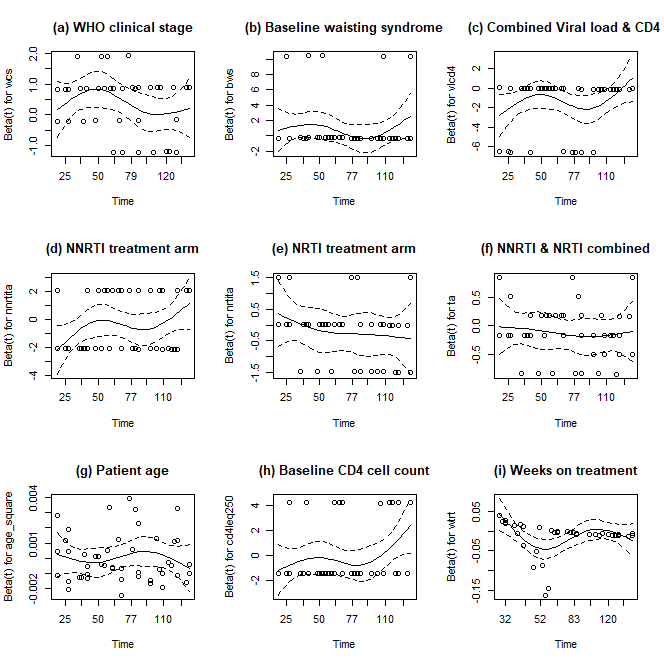
\includegraphics[width=\linewidth, keepaspectratio]{fig1.png}
%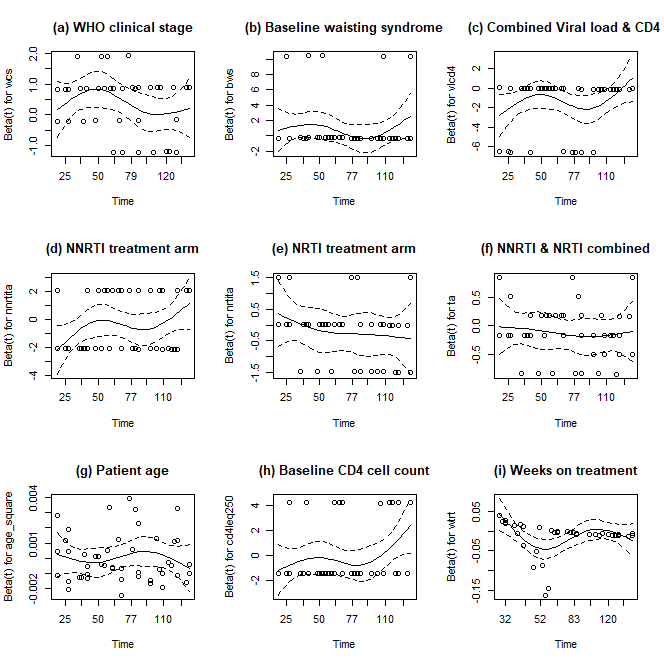
\includegraphics[width=\columnwidth]{fig1.png}  % scale to column width
%\caption{Plots of Schoenfeld residuals against time (weeks on treatment) %for the variables in the fitted Cox proportional hazards model.}
%\label{fig:1}
%\end{figure}

\begin{figure}[!htbp]
    \centering
    \subfloat[Body wasting syndrome]{\includegraphics[width=0.22\textwidth]{fig11a.pdf}}\hfill
    \subfloat[VL \& CD4]{\includegraphics[width=0.22\textwidth]{fig11b.pdf}}\\
    \subfloat[NNRTI]{\includegraphics[width=0.22\textwidth]{fig11c.pdf}}\hfill
    \subfloat[NRTI]{\includegraphics[width=0.22\textwidth]{fig11d.pdf}}\\
     \subfloat[NNRTI \& NRTI combined]{\includegraphics[width=0.22\textwidth]{fig11e.pdf}}\hfill
    \subfloat[Patient Age]{\includegraphics[width=0.22\textwidth]{fig11f.pdf}}\\
    \subfloat[Baseline CD4]{\includegraphics[width=0.22\textwidth]{fig11g.pdf}}\hfill
    \subfloat[WHO clinical stage]{\includegraphics[width=0.22\textwidth]{fig11h.pdf}}
    \caption{Plots of Schoenfeld residuals against time (weeks on treatment) for the variables in the fitted Cox proportional hazards model}
    \label{fig:1}
\end{figure}




\subsection{Fitting the Random Survival Forest Model}
The RSF is fitted using two splitting rules, the log-rank and the log-rank score and varying number of trees. Initially, the two forests were fitted using all the variables presented in Appendix 3, and the error rates from the out-of-bag (OOB) sample were 0.3193 and 0.3197 from the log-rank score and the log-rank, respectively. In Appendix 1, we present the plot of the OOB error rate against the number of trees. The plot shows that an optimal number of trees is reached when 80 trees are used, implying that adding more trees provides negligible improvement in the performance but increases computational cost. Next, we fitted the two models with all the values that were significant (p-value<0.05), from the Mantel-Haenszel test. We present the characteristics of the two forests in Table \ref{tab:table4} below. The error rates from the reduced RSF models based on the log-rank and the log-rank score were 0.2938 and 0.2936, respectively. This means that the percentage of misclassified instances by the RSF model is 29.4\%, resulting in a percentage accuracy of around 70.6\%. Thus, the fitted model generalises well to unseen data. These error rates are lower than those from the models with all the covariates. This contradicts findings from a study by \cite{Nasejje2017}, who argued that error rates decrease with the addition of more covariates. The c-index for the RSF model built from 80 trees has the highest index of 0.7141. This c-index falls in the acceptable range, between 0.7 and 0.8. This agrees with the results presented in Appendix 1, that 80 is the optimal number of trees. This is evidence that the model has some discriminatory ability. In addition, from the fitted RSF models, the continuous ranked probability score (CRPS) is approximately 0.03. This CRPS value is low, indicating that the predicted probability distribution matches the actual observed event time. 

\begin{table*}[t]
\centering
\caption{Characteristics of the fitted forest based on the log-rank and log-rank score splitting rules using a varying number of trees.}
\label{tab:table4}
\begin{tabular}{|p{5.5cm}|c|c|c|c|}
\hline
\multicolumn{1}{|c|}{} & \multicolumn{4}{|c|}{Splitting rule (Number trees)} \\
\cline{2-5}
\multicolumn{1}{|c|}{} & Logrank(500) & Logrankscore(500) & Logrank(100) & Logrank(80) \\
\hline
Sample size: & 613 & 613 & 613 & 613 \\
Number of virologic failure and resistance cases: & 41 & 41 & 41 & 41 \\
Number of trees: & 500 & 500 & 100 & 80 \\
Forest terminal node size: & 15 & 15 & 15 & 15 \\
Average no. of terminal nodes: & 18.815 & 22.546 & 19.08 & 19.3 \\
No. of variables tried at each split: & 4 & 4 & 3 & 3 \\
Total no. of variables: & 10 & 10 & 10 & 10 \\
Resampling used to grow trees: & Swor & Swor & Swor & Swor \\
Resample size used to grow trees: & 387 & 387 & 387 & 387 \\
Number of random split points: & 3 & 3 & 3 & 3 \\
(OOB) stand. CRPS: & 0.0310 & 0.0309 & 0.0312 & 0.0308 \\
(OOB) Requested performance error: & 0.292 & 0.294 & 0.293 & 0.286 \\
Concordance (c-index): & 0.708 & 0.706 & 0.707 & 0.714 \\
\hline
\end{tabular}
\end{table*}

\subsection{Variable Importance}
In Figure \ref{fig:2}, we present variable importance (VIMP) for the ten variables that were selected using the Mantel-Haenszel test. These ten variables were used to explain the probability of surviving from VFR, where Figure \ref{fig:2} helps to understand the ranking of feature importance and the magnitude of their impact. Graphs presented in Figure \ref{fig:2} show that the NRTI class of ART regimens has the greatest importance in predicting survival from VF and drug resistance. The NRTI, as presented earlier, is a class of drugs containing ZDV/3TC, ZDV/ddI, and D4T/3TC treatment regimens. Vlcd4 and Week on treatment are ranked as number 2 and 3, respectively. This is followed by the treatment arm (ta), which is a combination of the NRTI and the NNRTI (either NVP or EFV)) classes of drugs. Moreover, all variables have a non-zero importance to the probability of survival from VFR. However, a high variable importance does not necessarily imply the greatest impact. Therefore, we further extract the maximal subtree information to have a better understanding of the predictive strength of the variables using the first-order-depth and the second-order-depth.

\begin{figure}[H]
		%\begin{subfigure}
		\centering
        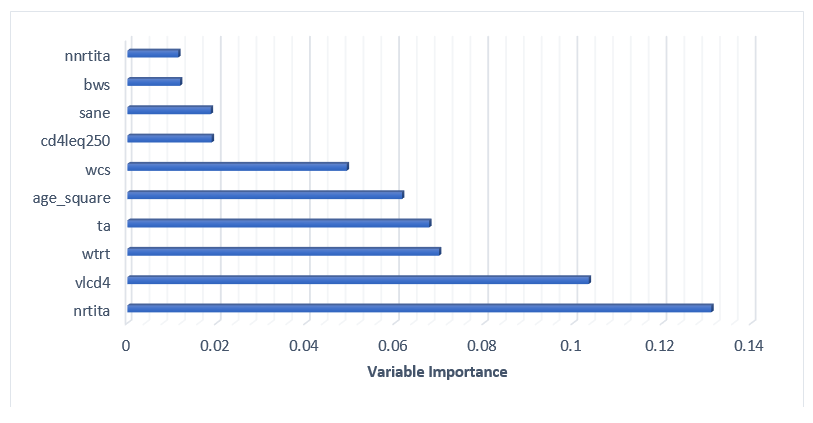
\includegraphics[width=\linewidth, keepaspectratio]{fig2.png}
		%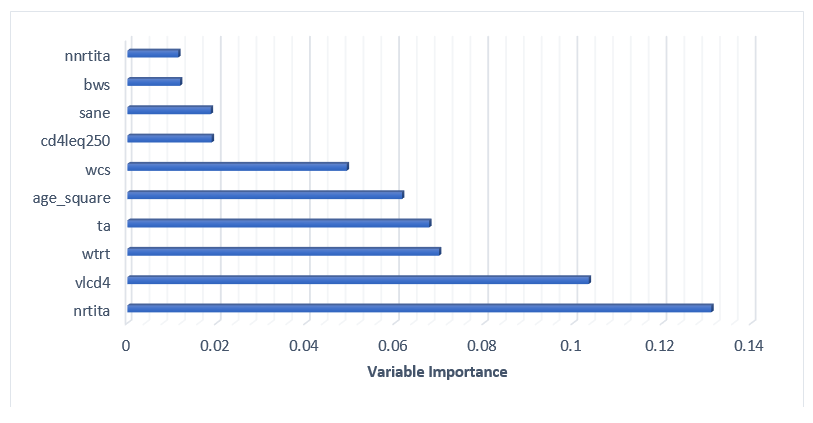
\includegraphics[height=2.8in, width=3.5in]{fig2.png}
		\caption{Rank of covariates based on how they influence virologic failure and drug resistance (VFR)}
		\label{fig:2}
	\end{figure}


\subsubsection{Acquire Maximal Subtree Information}
The first-order depth quantifies the predictive strength of a variable. It defines the distance from the root node to the parent of the closest maximal subtree for a variable. Smaller values indicate stronger predictive power. The second-order depth is the distance from the root to the second closest maximal subtree of the variable x. The first- and second-order-depth for the variables in the fitted model are presented in Table \ref{tab:virologic_failure}. 

\begin{table}[H]
    \centering
    \caption{First and Second order depths virologic failure and resistance}
    \label{tab:virologic_failure}
    \begin{tabular}{lcc}
        \toprule
        \textbf{Variable} & \textbf{First} & \textbf{Second} \\
        \midrule
        WHO clinical stage & 2.81 & 6.21 \\
        vlcd4 & 2.65 & 7.34 \\
        Baseline wasting syndrome & 4.21 & 7.55 \\
        Weeks on treatment & 2.62 & 6.33 \\
        Severe anemia & 3.53 & 6.92 \\
        NNRTI & 5.06 & 7.73 \\
        NRTI & 2.51 & 7.46 \\
        Treatment arm & 2.76 & 6.68 \\
        age\_square & 3.39 & 5.26 \\
        cd4\textless=250 & 4.89 & 6.95 \\
        \bottomrule
    \end{tabular}
\end{table}

Results in Table \ref{tab:virologic_failure} show that the NRTI class of regimens has the lowest first-order depth followed by week on treatment, vlowcd4, treatment arm (ta), and WHO clinical stage (wcs), in that order. The first-order depth for these variables is between 2.5 and 2.9. These variables have the strongest predictive power, in their order, compared to other variables. The NNRTI class of regimens has the highest first-order depth, meaning that it has the least predictive impact. To visualize the interactive tree for the variables, we plot the ensemble of trees, a hierarchical structure with terminal nodes highlighted with colour representing both the sample size and predicted value, where this value corresponds to the prediction from the selected tree and the sample size refers to the in-bag cases reaching a terminal point. Sample sizes represent all observations in- and out-of-bag cases. The ensemble of decision trees is presented in Figure \ref{fig:3}, and it starts with the variables, which have the most predictive power, that is, the NRTI class of ART regimens.

\begin{figure}[H]
		%\begin{subfigure}
		\centering
        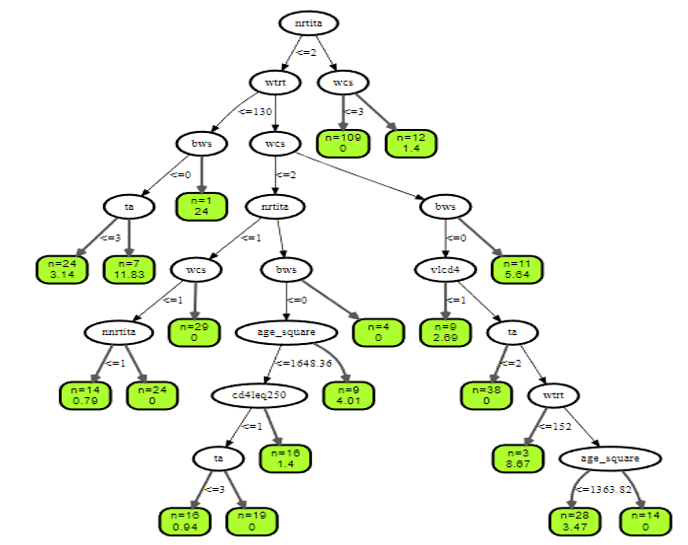
\includegraphics[width=\linewidth, keepaspectratio]{fig31.png}
		%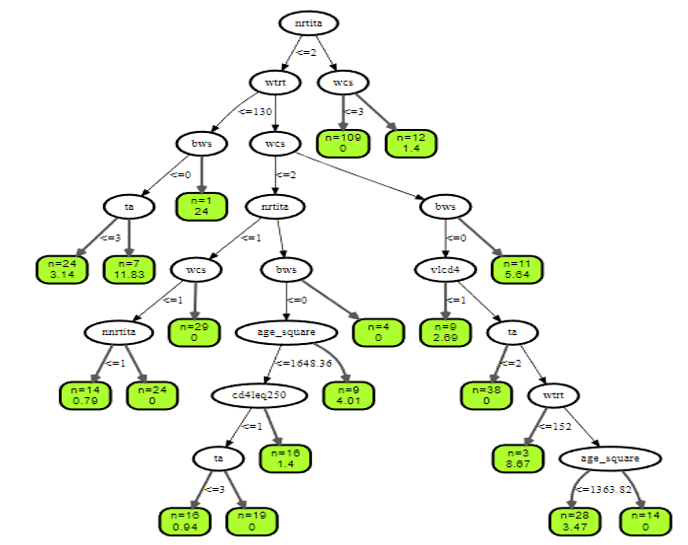
\includegraphics[height=3.7in, width=3.5in]{fig31.png}
		\caption{Ensemble of decision trees for the fitted RSF based on the log-rank splitting rule with 80 trees.}
		\label{fig:3}
	\end{figure}


The green rectangles in Figure \ref{fig:3} represent the terminal nodes of the ensemble tree. The terminal nodes present the number of individuals who fell into each of the final subgroups together with the estimated relative risk for that particular subgroup. These results are based on a sample size of 387 individuals, and these represent the training set. The results show that PLWHIV on treatment that includes NRTI class 1, that is D4T-3TC, and had no severe clinical stage (wcs$\leq 3$ had the highest survival from VF and drug resistance ($n=109; risk=0$). On the other hand, patients on NRTI classes 1 and 2 (ZDV-3TC and ZDV-ddI, respectively), being on treatment for less than 130 weeks and having a baseline wasting (bws=1) had the highest risk of virologic failure and drug resistance. Another interesting observation is that patients on NRTI class 1 (ZDV-3TC), at the asymptomatic WHO clinical stage and who were also administered NNRTI class 1 (NVP) were at a moderate risk of virologic failure and drug resistance. For this same subgroup, those on NNRTI class 2 were not at risk of virologic failure. Patience below the age of 41 years, CD4 baseline $\leq$ 250 and on treatment arm 4, 5 and 6 (EFV-ZDV-ddI, NVP-D4T-3TC, and EFV-D4T-3TC, respectively), had the lowest risk of virologic failure and drug resistance compared to those $\geq$ 41 years and those on treatment arm 1,2, and 3 (NVP-ZDV-3TC, EFV-ZDV-3TC, and NVP-ZDV-ddI, respectivel). Results in Figure \ref{fig:3} also show how interactions between variables affect survival outcomes. For example, baseline wasting syndrome and vlcd4 (viral load/CD4), the risk changes for those with bws = 0 where vlcd4 becomes the decisive factor. The predictive power of the age variable is also highly conditional on the NRTI, weeks on treatment, WHO clinical stage, and body wasting syndrome.


\subsubsection{Survival Estimates}
The main goal of survival analysis is to understand the probabilities of survival at different time points for all the individuals in a particular cohort. In a RSF model, an overall ensemble survival and the Nelson-Aalen estimator can be presented, and these results are shown in Figure \ref{fig:4} together with the Brier score, continuous-rank probability score (CRPS)= Brier score divided by time, and the plot of VF and drug resistance (VFR) for each individual. A Brier score of 0 means perfect, 1 means poor, and 0.25 means guessing, and stratifies these scores into groups that correspond to the 0-25, 25-50, 50-75, and 75-100 percentile values of VFR.

\begin{figure}[H]  % top of the column
\centering
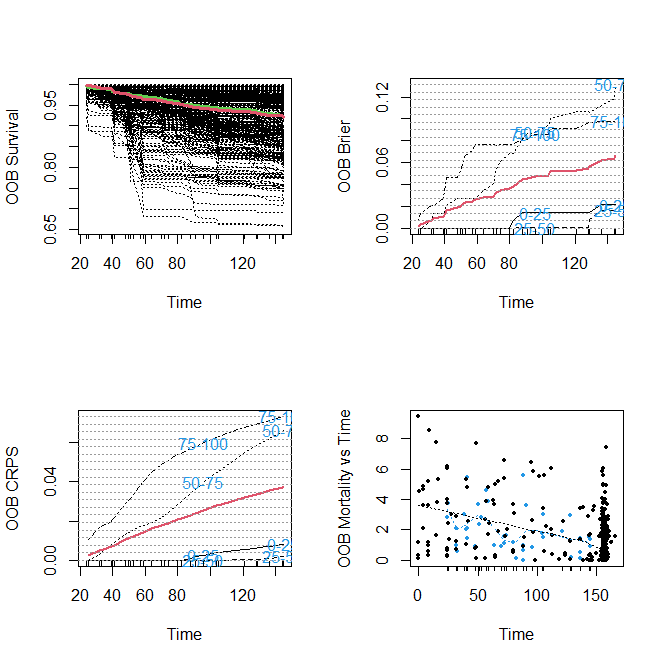
\includegraphics[width=\linewidth, keepaspectratio]{fig4.png}
%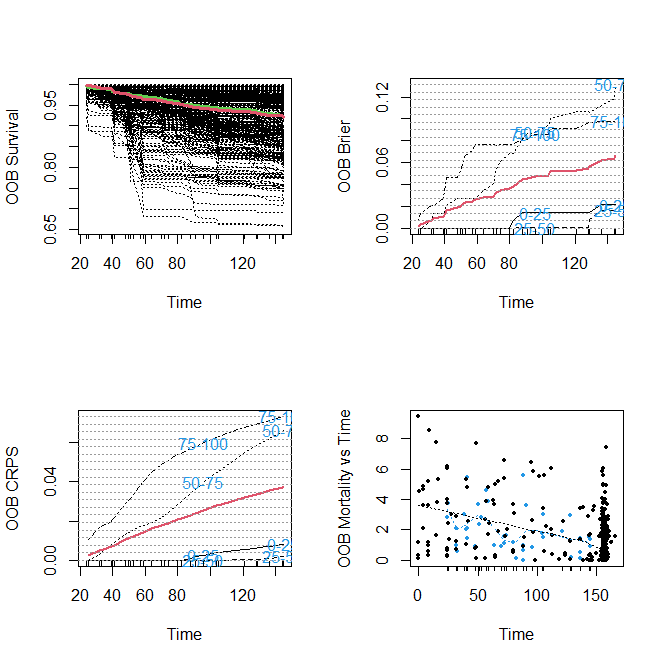
\includegraphics[width=\columnwidth]{fig4.png}  % scale to column width
\caption{Plots of survival estimates: Top left—Forest estimated survival function for each individual (thick red line is overall ensemble and thick green line is the Nelson-Aalen estimator); Top right—Brier score (0-poor, 1-perfect, 0.25-guessing); Bottom left—Continuous rank probability score (CRPS); Bottom right—Plot of mortality (virologic failure and resistance) for each individual.}
\label{fig:4}
\end{figure}


Figure \ref{fig:4}: Plots of survival estimates: Top left- Forest estimated survival function for each individual (thick red line is overall ensemble and thick green line is the Nelson-Aalen estimator); Top right- Brier score(0-poor, 1-perfect, 0.25-guessing); Bottom left-Continuous rank probability score (CRPS); Bottom right-Plot of mortality (virologic failure and resistance) for each individual.

The plot of the survival estimates, located at the top left, shows that the survival probabilities for each individual were above 65\%, and the overall ensemble survival (thick red line) for all individuals was above 90\% by the end of the study. The Nelson-Aalen method also gives estimates that are almost like the ones from the ensemble survival probabilities. The Brier scores on the top right in Figure 3 for the 0-25 and 25-50 percentiles are below 0.02, a value close to zero, for the entire follow-up period. This shows a perfect stratum. Although the Brier score for the 50 -75 percentile increases at a faster rate than the rest of the percentiles, it is below 0.12 for the entire period. The red line representing the overall (non-stratified) increases gradually up to around 0.06, which is closer to zero. The bottom left of Figure 3 shows a plot of the CRPS, which is equal to the integrated Brier score divided by time. The overall CRPS is below 0.04 for the entire period, which indicates accurate prediction. The last plot (bottom right) is the plot of VFR for each of the individuals. It shows the blue points that represent the event, VFR, and the black points representing censored observations. The blue line shows that VFR were high during the first weeks of the study, but a decreasing trend followed afterwards.

Appendix 2 represents the Brier score for the RSF model and that of the Kaplan-Meier estimates. From the first week of follow-up to around week 50, the Brier scores for the two models were the same. From week 50 to week 80, the Brier score for the Kaplan Meier estimates was lower than that of the RSF. From week 80 up to the end of the study, the Brier score for the RSF was lower than that of the Kaplan-Meier. This shows that the RSF performs better in the long-run compared to the traditional Kaplan-Meier method.

\subsubsection{Marginal effects of explanatory variables on VFR and survival from VFR}
To visualize how different levels of each variable, while holding other variables constant, affect the probability of survival from VFR, we present the marginal plots for the standardized VFR (mortality) in Figure \ref{fig:5}. In these plots, mortality represents our event of interest, which is VFR.


\begin{figure}[!htbp]
    \centering
    \subfloat[WHO clinical stage]{\includegraphics[width=0.22\textwidth]{fig66a.pdf}}\hfill
    \subfloat[Combined VL \& CD4]{\includegraphics[width=0.22\textwidth]{fig66b.pdf}}\\
    \subfloat[NRTI]{\includegraphics[width=0.22\textwidth]{fig66c.pdf}}\hfill
    \subfloat[Baseline wasting syndrome]{\includegraphics[width=0.22\textwidth]{fig66d.pdf}}\\
     \subfloat[Baseline CD4]{\includegraphics[width=0.22\textwidth]{fig66e.pdf}}\hfill
    \subfloat[NNRTI]{\includegraphics[width=0.22\textwidth]{fig66f.pdf}}\\
    \subfloat[Combined NNRTI \& NRTI]{\includegraphics[width=0.22\textwidth]{fig66g.pdf}}\hfill
    \subfloat[Weeks on Treat]{\includegraphics[width=0.22\textwidth]{fig66h.pdf}}
    \caption{Standardised VFR (presented by default as mortality in the plots) for different levels of each of the explanatory variables while holding other variables constant.}
    \label{fig:5}
\end{figure}


The NRTI treatment arm 2, which is ZDV/ddI, has the highest standardised VFR, followed by NRTI treatment arm 1, ZDV/3TC. NRTI treatment arm 3, D4T/3TC has the lowest standardised VFR. Six treatment arms (ta) were administered, and these were a combination of the NRTI class and the NNRTI class. 

Treatment arm 5, a combination of d4T/3TC (NRTI=3) and NVP (NNRTI=1), and treatment arm 6, a combination of d4T/3TC (NRTI=3) and EFV (NNRTI=2), had the lowest standardised VFR. However, treatment arm 3, a combination of ZDV/3TC (NRTI=1) and EFV, had the highest standardised VFR, followed by treatment arm 4, a combination of d4T/3TC and EFV. Treatment arm 3 contains ZDV/ddI and NVP, which has proved to have the highest standardised VFR among the NRTI class. The variable wtrt represents weeks on treatment. The results show a constant standardised VFR for the first 50 weeks on treatment, and afterwards it started to decrease exponentially. All values fall within the confidence bound, meaning that it is a perfect fit. Individuals who had a WHO clinical stage (wcs) of 4 at the randomisation stage had the highest standardised VFR, followed by individuals who had a WHO stage baseline of 3. Stage 4 is the advanced stage of HIV progression. WHO clinical stages 1 and 2 had the best outcome. A baseline CD4 cell count less than or equal to 250cell/mm$^3$ had higher VFR compared to individuals who had a CD4$>$ 250 at randomization. Furthermore, having severe anaemia (sane) during treatment leads to higher VFR compared to those patients who had no severe anaemia. The same goes for patients with baseline wasting syndrome (BWS). A combined effect of a CD4 cell count below 250 and a viral load above 10,000 (vlcd4=1) lead to a higher risk of VFR compared to individuals with recovered immunity and suppressed viral load (vlcd4=2). Figure 5 below presents the predicted survival from VFR for each of the covariates. Since survival is the opposite of mortality, the results presented in Figure 5 are the opposite of those presented in Figure \ref{fig:6}.

\begin{figure}[!htbp]
    \centering
    \subfloat[WHO clinical stage]{\includegraphics[width=0.22\textwidth]{fig55a.pdf}}\hfill
    \subfloat[Combined VL \& CD4]{\includegraphics[width=0.22\textwidth]{fig55b.pdf}}\\
    \subfloat[NRTI]{\includegraphics[width=0.22\textwidth]{fig55c.pdf}}\hfill
    \subfloat[Baseline wasting syndrome]{\includegraphics[width=0.22\textwidth]{fig55d.pdf}}\\
     \subfloat[Baseline CD4]{\includegraphics[width=0.22\textwidth]{fig55e.pdf}}\hfill
    \subfloat[NNRTI]{\includegraphics[width=0.22\textwidth]{fig55f.pdf}}\\
    \subfloat[Combined NNRTI \& NRTI]{\includegraphics[width=0.22\textwidth]{fig55g.pdf}}\hfill
    \subfloat[Weeks on Treat]{\includegraphics[width=0.22\textwidth]{fig55h.pdf}}
    \caption{Predicted Survival from VFR for each of the variables while holding other variables constant.}
    \label{fig:6}
\end{figure}


\subsubsection{Identifying pairwise interactions in the fitted Random Survival Forest }
We find pairwise interactions between variables using two approaches: the maximum subtree approach and the variable importance (VIMP) approach. The maximum subtree returns a matrix where entries [i][i] are the normalized minimal depth of variable [i] relative to the root node (normalized week on treatment the size of the tree) and entries [i][j] indicate the normalized minimal depth of a variable [j] wrt the maximal subtree for variable [i] (normalized wrt the size of [i]’s maximal subtree). Smaller [i][i] entries indicate predictive variables. Small [i][j] entries having small [i][i] entries are a sign of an interaction between variable i and j (note: the user should scan rows, not columns, for small entries). The results are presented in Table \ref{tab:pairwise_interactions}.

\begin{table*}[t]  % spans both columns
\centering
\scriptsize  % reduce font to fit
\caption{Finding pairwise interactions using the maximum subtree approach}
\label{tab:pairwise_interactions}
\begin{tabular}{@{}l*{10}{c}@{}}
\toprule
\textbf{Variable} & \textbf{nrtita} & \textbf{vlcd4} & \textbf{wtrt} & \textbf{wcs} & \textbf{ta} & \textbf{age\_square} & \textbf{sane} & \textbf{bws} & \textbf{cd4leq250} & \textbf{nnrtita} \\
\midrule
\textbf{nrtita} & 0.30 & 0.69 & 0.55 & 0.60 & 0.62 & 0.54 & 0.67 & 0.78 & 0.73 & 0.74 \\
\textbf{vlcd4} & 0.75 & 0.32 & 0.62 & 0.66 & 0.71 & 0.61 & 0.76 & 0.80 & 0.77 & 0.83 \\
\textbf{wtrt} & 0.76 & 0.78 & 0.32 & 0.68 & 0.71 & 0.57 & 0.77 & 0.74 & 0.73 & 0.79 \\
\textbf{wcs} & 0.80 & 0.83 & 0.63 & 0.33 & 0.72 & 0.58 & 0.76 & 0.84 & 0.75 & 0.78 \\
\textbf{ta} & 0.82 & 0.78 & 0.57 & 0.64 & 0.34 & 0.60 & 0.75 & 0.74 & 0.70 & 0.77 \\
\textbf{age\_square} & 0.86 & 0.90 & 0.74 & 0.74 & 0.77 & 0.40 & 0.89 & 0.89 & 0.80 & 0.87 \\
\textbf{sane} & 0.86 & 0.88 & 0.73 & 0.71 & 0.73 & 0.66 & 0.42 & 0.86 & 0.82 & 0.85 \\
\textbf{bws} & 0.85 & 0.85 & 0.70 & 0.79 & 0.80 & 0.75 & 0.86 & 0.52 & 0.84 & 0.87 \\
\textbf{cd4leq250} & 0.94 & 0.95 & 0.85 & 0.86 & 0.88 & 0.81 & 0.94 & 0.96 & 0.58 & 0.89 \\
\textbf{nnrtita} & 0.93 & 0.93 & 0.75 & 0.77 & 0.88 & 0.79 & 0.88 & 0.90 & 0.85 & 0.59 \\
\bottomrule
\end{tabular}
\end{table*}


Two variables are paired, and their paired VIMP is calculated (referred to as ’Paired’ importance). The VIMP for each separate variable is also calculated. The sum of these two values is referred to as ’Additive’ importance. A large positive or negative difference between ’Paired’ and ’Additive’ indicates an association worth pursuing if the univariate VIMP for each of the paired variables is reasonably large. The paired VIMP is calculated using the permute type of noise, and the results are presented in Table \ref{tab:interactions}.

\begin{table*}[t]
    \centering
    \caption{Identifying interactions using the variable importance approach}
    \label{tab:interactions}
    \begin{tabular}{@{}lccccc@{}}
        \toprule
        \textbf{Var 1:Var 2} & \textbf{Var 1} & \textbf{Var 2} & \textbf{Paired} & \textbf{Additive} & \textbf{Difference} \\
        \midrule
        nrtita:ta           & 0.0591 & 0.0384 & 0.1112 & 0.0975 & 0.0137 \\
        nrtita:wtrt         & 0.0591 & 0.0263 & 0.0785 & 0.0854 & -0.0069 \\
        nrtita:vlcd4        & 0.0591 & 0.0101 & 0.0712 & 0.0692 & 0.0020 \\
        nrtita:wcs          & 0.0591 & 0.0014 & 0.0750 & 0.0605 & 0.0145 \\
        nrtita:age\_square  & 0.0591 & 0.0078 & 0.0667 & 0.0670 & -0.0003 \\
        nrtita:sane         & 0.0591 & 0.0044 & 0.0716 & 0.0635 & 0.0080 \\
        nrtita:bws          & 0.0591 & 0.0018 & 0.0684 & 0.0610 & 0.0074 \\
        nrtita:nnrtita      & 0.0591 & 0.0094 & 0.0543 & 0.0685 & -0.0143 \\
        nrtita:cd4$\leq$250    & 0.0591 & 0.0013 & 0.0563 & 0.0604 & -0.0041 \\
        ta:wtrt             & 0.0352 & 0.0248 & 0.0517 & 0.0600 & -0.0083 \\
        ta:vlcd4            & 0.0352 & 0.0061 & 0.0490 & 0.0413 & 0.0076 \\
        ta:wcs              & 0.0352 & 0.0076 & 0.0566 & 0.0428 & 0.0139 \\
        ta:age\_square      & 0.0352 & 0.0028 & 0.0605 & 0.0380 & 0.0225 \\
        ta:sane             & 0.0352 & 0.0008 & 0.0491 & 0.0360 & 0.0131 \\
        ta:bws              & 0.0352 & -0.0037 & 0.0212 & 0.0315 & -0.0102 \\
        ta:nnrtita          & 0.0352 & -0.0016 & 0.0504 & 0.0336 & 0.0168 \\
        ta:cd4$\leq$250        & 0.0352 & 0.0064 & 0.0417 & 0.0416 & 0.0001 \\
        wtrt:vlcd4          & 0.0277 & 0.0152 & 0.0256 & 0.0428 & -0.0173 \\
        wtrt:wcs            & 0.0277 & 0.0074 & 0.0449 & 0.0350 & 0.0098 \\
        wtrt:age\_square    & 0.0277 & 0.0017 & 0.0200 & 0.0294 & -0.0094 \\
        wtrt:sane           & 0.0277 & 0.0009 & 0.0328 & 0.0285 & 0.0043 \\
        wtrt:bws            & 0.0277 & 0.0014 & 0.0323 & 0.0291 & 0.0032 \\
        wtrt:nnrtita        & 0.0277 & 0.0090 & 0.0294 & 0.0366 & -0.0073 \\
        wtrt:cd4$\leq$250      & 0.0277 & -0.0010 & 0.0315 & 0.0267 & 0.0048 \\
        vlcd4:wcs           & 0.0115 & 0.0130 & 0.0138 & 0.0246 & -0.0108 \\
        vlcd4:age\_square   & 0.0115 & 0.0064 & 0.0093 & 0.0179 & -0.0086 \\
        vlcd4:sane          & 0.0115 & -0.0010 & 0.0175 & 0.0105 & 0.0069 \\
        vlcd4:bws           & 0.0115 & -0.0020 & 0.0183 & 0.0095 & 0.0087 \\
        vlcd4:nnrtita       & 0.0115 & -0.0020 & 0.0136 & 0.0095 & 0.0041 \\
        vlcd4:cd4$\leq$250     & 0.0115 & 0.0058 & 0.0138 & 0.0174 & -0.0035 \\
        wcs:age\_square     & 0.0047 & 0.0112 & 0.0076 & 0.0159 & -0.0083 \\
        wcs:sane            & 0.0047 & 0.0058 & -0.0001 & 0.0105 & -0.0106 \\
        wcs:bws             & 0.0047 & -0.0034 & 0.0033 & 0.0013 & 0.0020 \\
        wcs:nnrtita         & 0.0047 & 0.0000 & 0.0228 & 0.0046 & 0.0181 \\
        wcs:cd4$\leq$250       & 0.0047 & 0.0082 & 0.0151 & 0.0128 & 0.0023 \\
        age\_square:sane    & 0.0004 & -0.0016 & 0.0065 & -0.0012 & 0.0077 \\
        age\_square:bws     & 0.0004 & 0.0003 & 0.0047 & 0.0007 & 0.0040 \\
        age\_square:nnrtita & 0.0004 & 0.0038 & 0.0045 & 0.0042 & 0.0003 \\
        age\_square:cd4$\leq$250 & 0.0004 & 0.0047 & 0.0169 & 0.0051 & 0.0118 \\
        sane:bws            & 0.0033 & 0.0020 & 0.0048 & 0.0053 & -0.0005 \\
        sane:nnrtita        & 0.0033 & 0.0059 & 0.0081 & 0.0092& -0.0012\\ % Data incomplete in prompt
        \bottomrule
    \end{tabular}
\end{table*}

Results in Tables \ref{tab:pairwise_interactions} and \ref{tab:interactions} show that the pair-wise interaction between NRTI with WHO clinical stage, treatment arm, and age; WHO clinical stage (wcs) weeks on treatment (wtrt) and age; and many other interactions are highlighted in Table \ref{tab:pairwise_interactions} and \ref{tab:interactions}. Thus, for example, the treatment arm, together with weeks on treatment, contributes to the virologic outcome of a PLWH. The same goes for the combination of the NRTI class of regimens with the baseline WHO clinical stage.

\subsection{ Discussion of Results}
This study utilised a RSF model benchmarked to the Cox proportional hazards model to analyse the likelihood of VFR among PLWH on ART within the Tshepo cohort, a randomized factorial study in Botswana that was carried out from 2002 to 2007. Whereas the selection of influential variables for the Cox proportional hazards model are based on the assessment of the Schoenfeld residuals and p-values, the RSF uses the variable importance approach. This limitation of the has resulted in eliminating variables such as the treatment arm (a combination of NNRTI and NRTI) since it failed to satisfy the proportional hazards assumption which is a requirement for the Cox proportional hazards model. However, based on the VIMP assessment, treatment arm was ranked as the second most influential variable in the RSF model. The core of this study was on the treatment arm, hence the use of the Cox proportional hazards model could not yield any interesting results.

The RSF model exhibited high predictive accuracy, with ensemble survival estimates surpassing 90\% and consistently low Brier scores across all percentiles in this study. The findings exceed the 2-year survival rate of 87\% documented by \cite{Afrashteh2023} in Iran and the 67\% median survival reported by \cite{Isingo2007} during the pre-ART era in Tanzania.  Discrepancies are anticipated due to variations in treatment availability, timing, and cohort characteristics.  The current study demonstrated that survival prediction accuracy was further validated by continuous ranked probability scores (CRPS), reflecting strong model performance over time.  This is consistent with the findings of \cite{Pu2024}, who identified the significant impact of early ART on enhancing survival probabilities.  In contrast to the multivariate Cox models employed by Pu and Wu, the RSF approach utilised in this study facilitated improved interpretability of variable importance and interaction effects while avoiding rigid parametric assumptions.

Our results further indicated that the NRTI class of ART regimens and the allocated treatment arms were the most important factors that predicted VFR. Therefore, the combination of ZDV and ddI in treatment arms that combines NVP/ZDV/ddI and EFV/ZDV/ddI had the greatest likelihood of treatment failure. This conclusion supports past research that raised pharmacological concerns about didanosine (ddI) affecting the mitochondria. Similarly, \cite{Nigussie2020} reported particular medication combinations and late presentation as the major reasons for treatment failure. On the other hand, treatment arms 5 and 6, which comprised the D4T/3TC combinations, had the greatest survival rates, despite the reported long-term toxicity of stavudine (D4T). These results show how important it is to assess the trade-off between early viral suppression and long-term tolerability when establishing the best treatment plans in resource-limited settings. 

Additionally, we found that various clinical and demographic characteristics are important, in addition to pharmacological predictors. A lower starting CD4 count ($\leq$250 cells/mm$^3$), severe anemia, being at WHO clinical stage 4, and having baseline wasting syndrome all significantly increased the risk of treatment failure. These findings are aligned with what \cite{Afrashteh2023}, \cite{Pu2024}, and \cite{Naghibifar2024} observed. All studies found that advanced clinical staging and immunosuppression at ART initiation were signs of severe outcomes. It is intriguing that certain studies, like \cite{Nigussie2020}, found adherence and opportunistic infections (like TB) to be crucial, yet these parameters weren't statistically significant in the present RSF model. The cohorts may differ, or the RSF may better account for covariate interactions and non-linear effects.

Furthermore, we also found important pairwise interactions using both the maximum subtree depth and the variable importance (VIMP) approaches. The most important interaction was between the NRTI class and the treatment arm. This supports the concept that ARV regimens should be looked at together, not separately, because there were also similar synergistic correlations between the number of weeks on treatment and CD4 levels and between the WHO clinical stage and the NNRTI class. These relationships show that the effectiveness of therapy does not only rely on clinical measures but also on how these markers interact with drug regimens. This understanding supports the personalised treatment strategy that \cite{Shaik2025} espouse by showing that a late diagnosis affects clinical staging. Finally, the RSF model shows how valuable it is for helping to create stratified HIV treatment plans in real-world situations.

The conclusions from these results are dual. First, they have significant ramifications for Botswana's HIV care and treatment plans. The discovery of important signs that can predict VFR, such as low baseline CD4 count, WHO clinical stage 4, severe anaemia, and baseline wasting syndrome, shows that it is important to identify PLWH at risk early on. This implies that PLWH displaying these risk factors should be given priority for more frequent VL assessments, targeted adherence counselling, and enhanced clinical monitoring, especially during the first three to six months of treatment, in a healthcare system where universal test-and-treat is the norm. Furthermore, the early peak in treatment failure that has been noticed emphasises how crucial the first treatment phase is, indicating that the national ART program might improve treatment outcomes by allocating more resources and assistance at this vulnerable time.

Second, the consequences for medication policy and the choice of ART regimen are equally important. Strong evidence supports updating treatment recommendations to reduce or completely avoid the use of ZDV/ddI-containing regimens due to the greater failure rates linked to these regimens (particularly Treatment Arms 3 and 4). This is especially true when there are more effective options. Despite being generally avoided because of long-term toxicity concerns, stavudine (D4T) may still be useful in some therapeutic circumstances under careful observation, as seen by its connection with better short-term virologic results in this group. The research also shows how machine learning models, like the RSF, may be used to support evidence-based decision-making. By improving viral suppression and lowering the spread of drug-resistant HIV strains, integrating such models into national health information systems could help physicians with real-time patient risk profiling, optimise resource allocation, and significantly advance Botswana's commitment to the UNAIDS 95-95-95 targets.

\section{Conclusion, Limitations, and Recommendations}
In this study, we effectively analysed drug resistance and time-to-VFR among Botswana patients on ART using a RSF model. Our method found key clinical and pharmacological markers, such as the NRTI medication class, treatment regimen, low baseline CD4 count, WHO stage 4 and severe anemia, which also showed good predictive precision. We further emphasized that the likelihood of survival increases with time, and VF often happens sooner in therapy. These results highlight the value of machine learning in survival analysis, especially when it comes to identifying interactions and non-linear effects that are difficult to identify using conventional Cox regression models.

Despite its strengths, the study has several limitations. The relatively small number of observed failure events (41 out of 613 PLWH) may affect the model’s generalizability and risk of overfitting. Additionally, while RSF models provide robust predictive insights, they do not yield hazard ratios, which limits interpretability for clinical audiences accustomed to classical regression charts. The study was also limited to a single cohort (Tshepo study) without external validation, which may restrict the applicability of the findings to broader HIV populations or other geographic settings. Furthermore, some known risk factors, such as adherence and opportunistic infections, did not emerge as significant in the model, which may be due to limitations in variable measurement or sample distribution.

Based on what we found, we suggest that Botswana's HIV program investigate adding risk-based methods to the procedures for starting and keeping track of ART. PLWH with high-risk clinical profiles should get extra help early on, such as more regular VL monitoring and adherence interventions throughout the first six months of therapy. We should phase out or use with caution drug regimens that are more likely to fail virologically, especially those that involve ZDV/ddI. Also, adding RSF models to national electronic health systems might make it easier to get real-time clinical decision assistance, which would lead to more personalised and data-driven HIV treatment. To ensure the RSF model is strong and applicable in other contexts, future studies should use larger, more diverse groups.

Limitations of the RSF model for this study is difficulty handling time-varying covariates without extensions, a potential violation of the proportional hazards assumption by the log-rank split statistic, challenges in processing complex survival, longitudinal, and multivariate (SLAM) outcomes, and the possibility of overfitting if too many features are present in the dataset. We would recommend that future studies capture longitudinal variables (eg CD4 cell counts, and viral load) and use newer methodologies like RF-SLAM by using Poisson regression log-likelihood as a split statistic to include time-varying predictors and handle SLAM data


\section*{Acknowledgement}
The authors acknowledge the reviewers for their invaluable comments that helped improve our paper.

\noindent The authors are grateful to the anonymous referee for a careful
checking of the details and for helpful comments that improved this
paper.

\section*{FUNDING}
CS was supported by the University of Botswana, Department of Statistics. SM and OTC were supported through the Sub-Saharan African Network for TB/HIV Research Excellence (SANTHE 3.0) from the Bill and Melinda Gates Foundation (INV-033558). OTC was supported by the Fogarty International Center at the US National Institutes of Health (D43 TW009610). SM was partially supported by the Fogarty International Center at the US National Institutes of Health (K43TW 012350). SM \& OTC were supported by the TESAIII of Excellence in Southern Africa (TESA III), which is part of the EDCTP2 program supported by the European Union (CSA2020NoE-3104 TESAIII of Excellence in Southern Africa (TESA III), which is part of the EDCTP2 program supported by the European Union (CSA2020NoE-3104 TESAIII CSA2020NoE). The views expressed in this publication are those of the authors and not necessarily those of the funding agencies. The funders had no role in the study design, data collection, decision to publish, or preparation of this manuscript.


\begin{thebibliography}{99}

	\bibitem{UNAIDS2024} 
UNAIDS, Global HIV \& AIDS statistics — Fact sheet (2024). \url{https://www.unaids.org/en/resources/fact-sheet.}. 

\bibitem{WHO2023} 
World Health Organisation. HIV/AIDS Report. 2023. \url{https://www.afro.who.int/health-topics/hivaids}

\bibitem{Bareng2024}
Bareng, O. T., Moyo, S., Mudanga, M., Sebina, K., Koofhethile, C. K., Choga, W. T., Moraka, N. O., Maruapula, D., Gobe, I., Motswaledi, M. S., Musonda, R., Nkomo, B., Ramaabya, D., Chebani, T., Makuruetsa, P., Makhema, J., Shapiro, R., Lockman, S., \& Gaseitsiwe, S. (2024). Low-Level Viremia among Adults Living with HIV on Dolutegravir-Based First-Line Antiretroviral Therapy Is a Predictor of Virological Failure in Botswana. Viruses, 16(5), 720. \url{https://doi.org/10.3390/v16050720}

\bibitem{Daltro2023} 
Borges Daltro, A. C., Almeida, C. S., Costa Unfried, A. G., \& Álvares Travassos, A. G. (2023). Virological failure and adherence to antiretroviral therapy in adolescents and young adults living with human immunodeficiency virus. Tropical Medicine \& International Health, 28(3), 162-174. \url{https://doi.org/10.1111/tmi.13854}.




\bibitem{Ekstrand2011}
Ekstrand, M. L., Shet, A., Chandy, S., Singh, G., Shamsundar, R., Madhavan, V., Saravanan, S., Heylen, E., \& Kumarasamy, N. (2011). Suboptimal adherence associated with virological failure and resistance mutations to first-line highly active antiretroviral therapy (HAART) in Bangalore, India. International Health, 3(1), 27. \url{https://doi.org/10.1016/j.inhe.2010.11.003}.


\bibitem{Bulage2017} 
Bulage L, Ssewanyana I, Nankabirwa V, Nsubuga F, Kihembo C, Pande G, Ario AR, Matovu JK, Wanyenze RK, Kiyaga C. Factors Associated with Virological Non-suppression among HIV-Positive Patients on Antiretroviral Therapy in Uganda, August 2014-July 2015. BMC Infect Dis. 2017 May 3;17(1):326. doi: 10.1186/s12879-017-2428-3. PMID: 28468608; PMCID: PMC5415758.

\bibitem{Chun2010} 
Chun T.W., Justement J.S., Murray D., Hallahan C.W., Maenza J., Collier A.C., Sheth P.M., Kaul R., Ostrowski M., Moir S., et al. Rebound of plasma viremia following cessation of antiretroviral therapy despite profoundly low levels of HIV reservoir: Implications for eradication. Aids. 2010;24:2803–2808. doi: 10.1097/QAD.0b013e328340a239.

\bibitem{Tobin2005} 
Tobin N.H., Learn G.H., Holte S.E., Wang Y., Melvin A.J., McKernan J.L., Pawluk D.M., Mohan K.M., Lewis P.F., Mullins J.I., et al. Evidence that low-level viremias during effective highly active antiretroviral therapy result from two processes: Expression of archival virus and replication of virus. J. Virol. 2005;79:9625–9634. doi: 10.1128/JVI.79.15.9625-9634.2005. 

\bibitem{Manakhov2025} 
Monakhov N.E., Sharipova E.A., Lapunova S.V., Vinogradova T.N., Lioznov D.A. Acquired drug resistance of HIV in patients with virological failure of first-line art. HIV Infection and Immunosuppressive Disorders. 2025;17(3):42-53. (In Russ.) \url{https://doi.org/10.22328/2077-9828-2025-17-3-42-53}.

\bibitem{Li2021} 
Li J.Z., Gallien S., Do T.D., Martin J.N., Deeks S., Kuritzkes D.R., Hatano H. Prevalence and significance of HIV-1 drug resistance mutations among patients on antiretroviral therapy with detectable low-level viremia. Antimicrob. Agents Chemother. 2012;56:5998–6000. doi: 10.1128/AAC.01217-12

\bibitem{Naghibifar2024}
Naghibifar, Z., Janbakhsh, A., Sajadipour, M., Emadzadeh, M., Naghipour, A., \& Sahebkar, A., Survival rate and its predictors in HIV patients: A 15-year follow-up of 3030 patients. \textit{Journal of Infection and Public Health}, 17(9), 102520, (2024). \url{https://doi.org/10.1016/j.jiph.2024.102520}.

\bibitem{Isingo2007}
Isingo, R., Zaba, B., Marston, M., Nakiyingi, J., Urassa, M., \& Todd, J. Survival after HIV infection in the pre-antiretroviral therapy era in a rural Tanzanian cohort. \textit{AIDS}, 21(Suppl 6), S5–S13, (2007). \url{https://doi.org/10.1097/01.aids}.0000299405.06658.a8.

\bibitem{Afrashteh2023}
Afrashteh, S., Fararouei, M., Ghaem, H., \& Gheibi, Z. Factors associated with progression from HIV to death in patients receiving antiretroviral therapy in Southern Iran: A 21-year survival analysis. \textit{HIV \& AIDS Review International Journal of HIV-Related Problems}, 22(3), 189–197, (2023). \url{https://doi.org/10.5114/hivar.2023.131466}

\bibitem{Pu2024}
Pu J-f and Wu J Survival analysis of PLWHA undergoing combined antiretroviral therapy: exploring long-term prognosis and influencing factors. \textit{Front. Public Health.} 12:1327264, (2024). doi: 10.3389/fpubh.2024.1327264.

\bibitem{Nigussie2020}
Nigussie, F., Alamer, A., Mengistu, Z., \& Tachbele, E.. Survival and predictors of mortality among adult HIV/AIDS patients initiating HAART in Ethiopia: A retrospective cohort study. \textit{HIV/AIDS – Research and Palliative Care}, 12, 757–768, (2020). \url{https://doi.org/10.2147/HIV.S274747}.

\bibitem{Nura2024} 
Nura GJ, Wario KS, Erango MA, Determinants of survival time for HIV/AIDS patients in the pastoralist region of Borena: a study at Yabelo General Hospital, South East Ethiopia. \textit{AIDS Res Th} 28;21(1):58 (2024). doi: 10.1186/s12981-024-00644-1. PMID: 39198844; PMCID: PMC11360864.

\bibitem{Shaik2025} 
Shaik, R.A., Holyachi, S.K., Ahmad, M.S. The impact of delay in HIV diagnosis on patient survival: analysis of HIV infection trends from 2007 to 2023. \textit{BMC Infect Dis} 25, 177 (2025). \url{https://doi.org/10.1186/s12879-024-10412-1}.

\bibitem{Nasejje2017} 
Nasejje, J.B., Mwambi, H., Application of random survival forests in understanding the determinants of under-five child mortality in Uganda in the presence of covariates that satisfy the proportional and non-proportional hazards assumption. \textit{BMC Res Notes} 10, 459 (2017). \url{https://doi.org/10.1186/s13104-017-2775-6}.

\bibitem{Ishwaran2008}
Ishwaran H, Kogalur U , Blackstone  E. H. and Lauer M.S.. Random Survival Forests, \textit{The Annals of Applied Statistics}, Vol. 2, No. 3, 841–860 (2008), DOI: 10.1214/08-AOAS169.

\bibitem{Berkowitz2023}
Berkowitz M, Altman RM, Loughin TM. Random forests for survival data: which methods work best and under what conditions? \textit{Int J Biostat.} Apr 24;20(2):315-345 (2024). \url{https://doi: 10.1515/ijb-2023-0056}. PMID: 38656274; PMCID: PMC11661562.

\bibitem{Bussmann2009} 
Bussmann H, Wester CW, Thomas A, Novitsky V, Okezie R, Muzenda T, Gaolathe T, Ndwapi N, Mawoko N, Widenfelt E, Moyo S, Musonda R, Mine M, Makhema J, Moffat H, Essex M, Degruttola V, Marlink RG. Response to zidovudine/didanosine-containing combination antiretroviral therapy among HIV-1 subtype C-infected adults in Botswana: two-year outcomes from a randomized clinical trial. \textit{J Acquir Immune Defic Syndr}.;51(1):37-46 (2009). doi: 10.1097/QAI.0b013e31819ff102. PMID: 19282782; PMCID: PMC3066172.

\bibitem{Breiman2003} 
Breiman, L. and Cutler, A. Setting up, using, and understanding random forests V4.0. \textit{Dept. Statistics, Univ. California, Berkeley} (2003)

\bibitem{Segal1988} 
SEGAL, M. R. Regression trees for censored data. \textit{Biometrics} 44 35–47 (1988).

\bibitem{Ishwaran2025} 
Ishwaran H, Kogalur U. Fast Unified Random Forests for Survival, Regression, and Classification (RF-SRC). R package version 3.4.1 (2025), \url{https://cran.r-project.org/package=randomForestSRC}

\end{thebibliography}


\newpage


\section{Appendices}
\subsection*{Appendix 1: The prediction error rate for a random survival forest of 500 trees suggesting an optimal number of trees equal to 80.}
\begin{figure}[H]  % top of the column
\centering
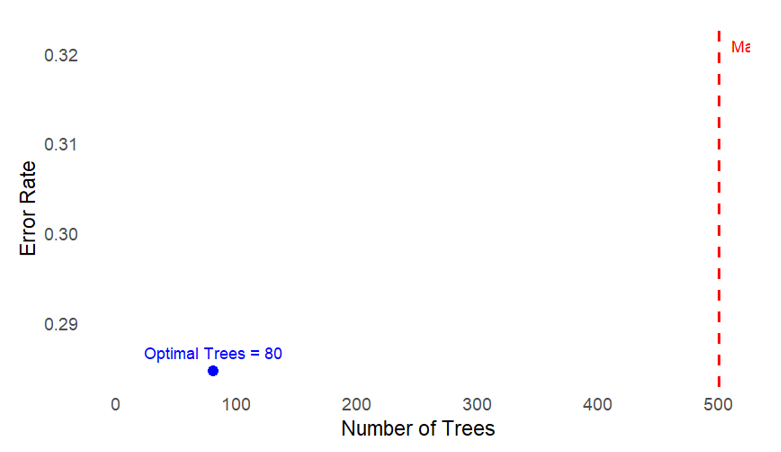
\includegraphics[width=\columnwidth]{appendix1.png}  % scale to column width
\label{fig:7}
\end{figure}



\subsection*{Appendix 2: Brier Score for the RSF model and Kaplan Meier estimates}
\begin{figure}[H]  % top of the column
\centering
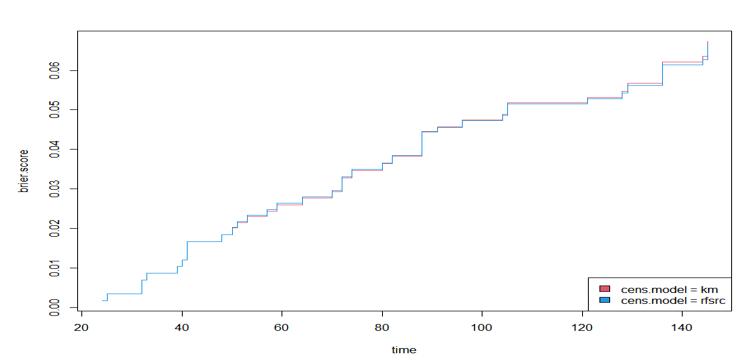
\includegraphics[width=\columnwidth]{appendix2.png}  % scale to column width
\label{fig:8}
\end{figure}

\newpage
%\subsection*{Appendix 3: Mantel-Haenszel Test for the association of %Virologic Failure with Resistance and Explanatory variables}

\begin{table*}[!htbp]
    \centering
    \caption{Mantel-Haenszel Test for the association of Virologic Failure with Resistance and Explanatory variables}\label{tab:appendix3}
    \begin{tabularx}{\textwidth}{@{}p{6.5cm} X c c c@{}}
        \toprule
        \textbf{Feature} & \textbf{Coding} & \textbf{Censored = 0 ($n$, \%)} & \textbf{Event = 1 ($n$, \%)} & \textbf{\textit{p}-value} \\
        \midrule
        \textbf{Gender} & 1: Male & 183 (28.2) & 16 (2.5) & 0.6000 \\
        & 2: Female & 419 (64.4) & 32 (4.9) &\\
        \addlinespace
        \textbf{WHO clinical stage (wcs)} & 1: Asymptomatic & 190 (30.0) & 8 (1.3)& 0.0300 \\
        & 2: Mild symptoms & 152 (24.0) & 9 (1.4)& \\
        & 3: Advanced  & 192 (30.3) & 24 (3.8) &\\
        & 4: Severe & 54 (8.5) & 4 (0.6) &\\
        \addlinespace
        \textbf{Baseline BMI} & 1: BMI $<$ 18.5 & 110 (17.0) & 11 (1.7) & 0.5592 \\
        & 2: 18.5 $\le$ BMI $<$ 24.9 & 358 (55.4) & 28 (4.3) & \\
        & 3: 24.9 $\le$ BMI $<$ 29.9 & 90 (13.9) & 8 (1.2) & \\
        & 4: BMI $\ge$ 29.9 & 40 (6.2) & 1 (0.2) & \\
        \addlinespace
        \textbf{Combined Viral load \& CD4 (vlcd4)} &  1: CD4 $<$ 250 \& VL $>$ 10,000 & 35 (5.4) & 9 (1.4) & 0.0002 \\
        & 2: CD4 $\ge$ 250 \& VL $\le$ 10,000 & 567 (87.2) & 39 (6.0)& \\
        \addlinespace
        \textbf{Baseline wasting syndrome (bws)} & 0: No & 573 (88.2) & 43 (6.6) & 0.0700 \\
        & 1: Yes & 29 (4.5) & 5 (0.8) & \\
        \addlinespace
        \textbf{Weeks on Treatment (wtrt)} & & & & $<$0.0001 \\
        \addlinespace
        \textbf{Moderate Anemia (mane) 10--12 gr/dL}  & 0: No & 356 (54.8) & 31 (4.8) & 0.5000  \\
        & 1: Yes & 246 (37.8) & 17 (2.6)& \\
        \addlinespace
        \textbf{CD4 strata} & 1: CD4 $\le$ 200 & 305 (46.9) & 25 (3.8) & 0.8000 \\
        & 2: CD4 $>$ 200 & 297 (45.7) & 23 (3.5)& \\
        \addlinespace
        \textbf{BMI below 18} & 0: No & 492 (75.7) & 37 (5.7)  & 0.5466 \\
        & 1: Yes & 110 (16.9) & 11 (1.7) & \\
        \addlinespace
        \textbf{Peripheral Neuropathy} & 0: No & 538 (82.8) & 42 (6.5) & 0.6000 \\
        & 1: Yes & 64 (9.8) & 6 (0.9) &\\
        \addlinespace
        \textbf{Baseline viral load above 100,000} & 0: No & 204 (31.4) & 12 (1.8) & 0.2000 \\
        & 1: Yes & 397 (61.2) & 36 (5.5)& \\
        \addlinespace
        \textbf{Severe anemia ($\ge$10 gr/dL)} & 0: No & 514 (79.1) & 35 (5.4) & 0.0369 \\
        & 1: Yes & 88 (13.5) & 13 (2.0) &\\
        \addlinespace
        \textbf{CD4 $\le$ 250} & 1: Yes & 446 (68.6) & 37 (5.7)& 0.0100 \\
        & 2: No & 156 (24.0) & 11 (1.7) & \\
        \addlinespace
        \textbf{Any TB} & 0: No & 551 (84.8) & 42 (6.5) & 0.1000 \\
        & 1: Yes & 51 (7.8) & 6 (0.9)& \\
        \addlinespace
        \textbf{Adherence} & 0: Yes & 299 (46.0) & 26 (4.0) & 0.6000 \\
        & 1: No & 303 (46.6) & 22 (3.3) &\\
        \addlinespace
        \textbf{Age$^2$} & & & & $<$0.0001 \\
        \addlinespace
        \textbf{NNRTI Treatment Arm (nnritta)} & 1: NVP & 296 (45.5) & 29 (4.5) & 0.1000 \\
        & 2: EFV & 306 (47.1) & 9 (0.3) &\\
        \addlinespace
        \textbf{NRTI Treatment Arm (nrtita)} & 1: ZDV/3TC & 207 (31.8) & 11 (1.7) & $<$0.0001 \\
        & 2: ZDV/ddI & 184 (28.3) & 32 (4.9)& \\
        & 3: d4T/3TC & 211 (32.5) & 5 (0.8) &\\
        \addlinespace
        \textbf{Treatment Arm (ta)} & 1: NVP/ZDV/3TC & 102 (15.7) & 7 (1.1)  & $<$0.0001 \\
        & 2: EFV/ZDV/3TC & 105 (16.2) & 4 (0.6) & \\
        & 3: NVP/ZDV/ddI & 88 (13.5) & 20 (3.1) & \\
        & 4: EFV/ZDV/ddI & 96 (14.7) & 12 (1.5) & \\
        & 5: NVP/D4T/3TC & 106 (16.3) & 2 (0.3) & \\
        & 6: EFV/D4T/3TC & 105 (16.2) & 3 (0.5) & \\
        \bottomrule
    \end{tabularx}
\end{table*}




\end{document}
